\documentclass[tikz,border=3pt]{standalone}

\usepackage{pgfplots}
\pgfplotsset{compat=1.15}

\usepackage{mathrsfs}
\usetikzlibrary{arrows}
\usetikzlibrary{patterns}
\usepackage{graphicx}

\begin{document}
	
	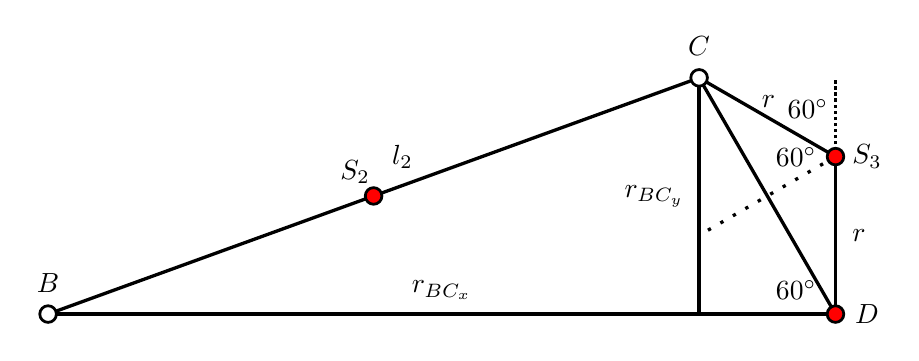
\begin{tikzpicture}
		
		% Alapvonal
		\draw [line width=1.2pt] (0,0)--(10,0); % alsó oldal
		
		% Háromszög oldalai
		\draw [line width=1.2pt] (10,0)--(10-1.732050807568877,2+1); % jobb oldal
		\draw [line width=1.2pt] (10-1.732050807568877,2+1)--(0,0); % bal oldal
		
		% Magasság és sugarak
		\draw [line width=1.2pt] (10-1.732050807568877,2+1)--(10-1.732050807568877,0); % magasság
		\draw [line width=1.2pt] (10,0)--(10,2); % alsó sugár
		\draw [line width=1.2pt] (10,2)--(10-1.732050807568877,2+1); % felső sugár
		
		% Segédvonalak
		\draw [line width=1.2pt, densely dotted] (10,2)--(10,3); % felfelé
		\draw [line width=1.2pt, loosely dotted] (10,2)--(10-1.732050807568877,2-1); % jobb magasság
		
		% Pontok és címkék
		\draw [fill=white, line width=1pt] (0,0) circle (3pt);
		\draw[color=black] (0,0.4) node {$B$};
		
		\draw [fill=red, line width=1pt] (10,0) circle (3pt);
		\draw[color=black] (10.4,0) node {$D$};
		
		\draw [fill=white, line width=1pt] (10-1.732050807568877,2+1) circle (3pt);
		\draw[color=black] (10-1.732050807568877,3.4) node {$C$};
		
		\draw [fill=red, line width=1pt] (4.13397459622,1.5) circle (3pt);
		\draw[color=black] (3.9,1.8) node {$S_2$};
		
		\draw [fill=red, line width=1pt] (10,2) circle (3pt);
		\draw[color=black] (10.4,2) node {$S_3$};
		
		% Szögek és jelölések
		\draw[color=black] (9.65,2.6) node {$60^\circ$};
		\draw[color=black] (9.5,2) node {$60^\circ$};
		\draw[color=black] (9.5,0.3) node {$60^\circ$};
		
		% Távolságok
		\draw[color=black] (4.5,2) node {$l_2$};
		\draw[color=black] (10.3,1) node {$r$};
		\draw[color=black] (9.15,2.7) node {$r$};
		\draw[color=black] (5,0.3) node {$r_{BC_x}$};
		\draw[color=black] (7.7,1.5) node {$r_{BC_y}$};
		
	\end{tikzpicture}
	
\end{document}
